\documentclass[sigconf,nonacm]{acmart}

\usepackage{amsmath}
\usepackage{graphicx}
\usepackage{booktabs}
\usepackage[inline]{enumitem}

\settopmatter{printacmref=false}
\renewcommand\footnotetextcopyrightpermission[1]{}
\pagestyle{plain}

\setcopyright{none}
\acmConference[]{}{}{}
\acmYear{2026}
\copyrightyear{2026}
\acmISBN{}
\acmDOI{}

\begin{document}

\title{The Traveling Flyerperson: An Introduction}
\subtitle{Where do I place these flyers in Cambridge, MA?}

\author{Cambridge Developers}
\affiliation{
  \country{USA}
  \city{Cambridge}
  \state{MA}
}

\renewcommand{\shortauthors}{Cambridge Developers}

\begin{abstract}
We introduce \emph{The Traveling Flyerperson}, a project that takes a simple civic question---where should a small software group place flyers in Cambridge, Massachusetts?---and uses it as a lens for exploring algorithms, geography, and decision-making. This primer presents the core ideas: the routing problem as a Traveling Salesman Problem, the legal and practical constraints of flyering in Cambridge, and the interactive web application that ties them together. We leave the full statistical framework (survival analysis, point processes, Bayesian hierarchical models) to the companion paper and focus here on motivation, setup, and what makes this problem interesting.
\end{abstract}

\keywords{Traveling Salesman Problem, civic computing, Cambridge MA, route optimization}

\maketitle

\section{The Problem}

You have a stack of flyers for a local software group. You live in Cambridge, Massachusetts---6.4 square miles of dense sidewalks, two research universities, and a long tradition of community bulletin boards. You want to post these flyers where people will actually see them, and you want to walk (or bike) an efficient route to do it.

This is a real problem we faced at \texttt{cambridge-dev.org}. It turns out to be more interesting than it looks.

\subsection{Why Not Just Walk?}

The naive approach---grab a stack, walk to familiar spots---works. But it raises questions you can't answer without thinking harder:

\begin{itemize}
    \item Are you visiting the \emph{best} locations, or just the ones you know?
    \item Is your route efficient, or are you backtracking?
    \item How long do flyers actually last before someone removes them?
    \item Are there legal constraints you're violating without knowing?
\end{itemize}

Each of these questions opens a door to a different area of computer science or statistics. The project walks through those doors one at a time.

\section{The Routing Problem}

Given $n$ locations to visit, starting and ending at the Cambridge Public Library, what's the shortest route? This is the Traveling Salesman Problem (TSP)---one of the most studied problems in combinatorial optimization.

For our purposes, the ``distance'' between two locations is the straight-line (Haversine) distance on the Earth's surface. A tour is a permutation $\pi$ of the locations with total cost:
\begin{equation}
    \mathcal{C}(\pi) = \sum_{i=1}^{n-1} d(\pi_i, \pi_{i+1}) + d(\pi_n, \pi_1)
\end{equation}
where $d(\cdot, \cdot)$ is the Haversine distance. We want the permutation that minimizes this cost.

\subsection{Three Approaches}

The application implements three solvers, each illustrating a different algorithmic strategy:

\paragraph{Brute Force.} Try every possible ordering. There are $(n-1)!/2$ distinct tours. For our $\sim$10 locations this is about 181,000 tours---feasible, but the approach collapses for larger inputs. This gives the \emph{exact} optimal solution.

\paragraph{Nearest Neighbor.} A greedy heuristic: from your current location, always go to the closest unvisited stop. Fast ($O(n^2)$) but often produces routes 20--30\% longer than optimal because it doesn't plan ahead.

\paragraph{2-Opt.} Start with the Nearest Neighbor solution, then iteratively improve it: pick two edges in the tour, reverse the segment between them, and keep the change if it shortens the route. Repeat until no improvement is found. This is a \emph{local search} method---it can't guarantee the global optimum, but in practice it gets close.

\section{The Constraints}

Cambridge isn't a blank grid. The problem has real-world constraints that make it more than a textbook exercise.

\subsection{Legal Rules}

Massachusetts law and Cambridge municipal code prohibit posting on:
\begin{itemize}
    \item Public utility poles and lamp posts
    \item Shade trees and public buildings
    \item Sidewalks and public infrastructure
\end{itemize}
The fine is \$300 per violation. This immediately eliminates the most visible, highest-traffic locations---the ones a naive flyerperson would target first.

\subsection{Permission and Policing}

Even on private property, most locations require permission. Cafes curate their boards. Libraries have posting policies. MIT reserves campus boards for recognized student groups. Business Improvement Districts (like Central Square) employ crews that remove unauthorized postings daily.

The net effect: the set of \emph{valid} flyering locations is much smaller than the set of \emph{visible} ones, and survival time varies enormously by location type.

\subsection{Geography}

Cambridge is bounded by the Charles River to the south, Somerville to the north, and Boston to the east. The road network, one-way streets, and pedestrian paths constrain actual walking routes in ways that straight-line distance doesn't capture. (A future version of this project will incorporate real walking distances via OSRM or GraphHopper.)

\section{The Application}

The deployed application at \texttt{letters-cambridge.web.app/stories/flyering/} is a static SvelteKit site that runs entirely in the browser. No backend, no accounts, no data collection.

\begin{figure}[t]
    \centering
    
\includegraphics[width=\linewidth]{figures/app-desktop.png}
    \caption{Desktop view. The sidebar exposes solver selection, route summary, legal rules, and toggleable map layers. The map shows the computed tour over Cambridge with CARTO dark tiles.}
    \label{fig:desktop}
\end{figure}

\begin{figure}[t]
    \centering
    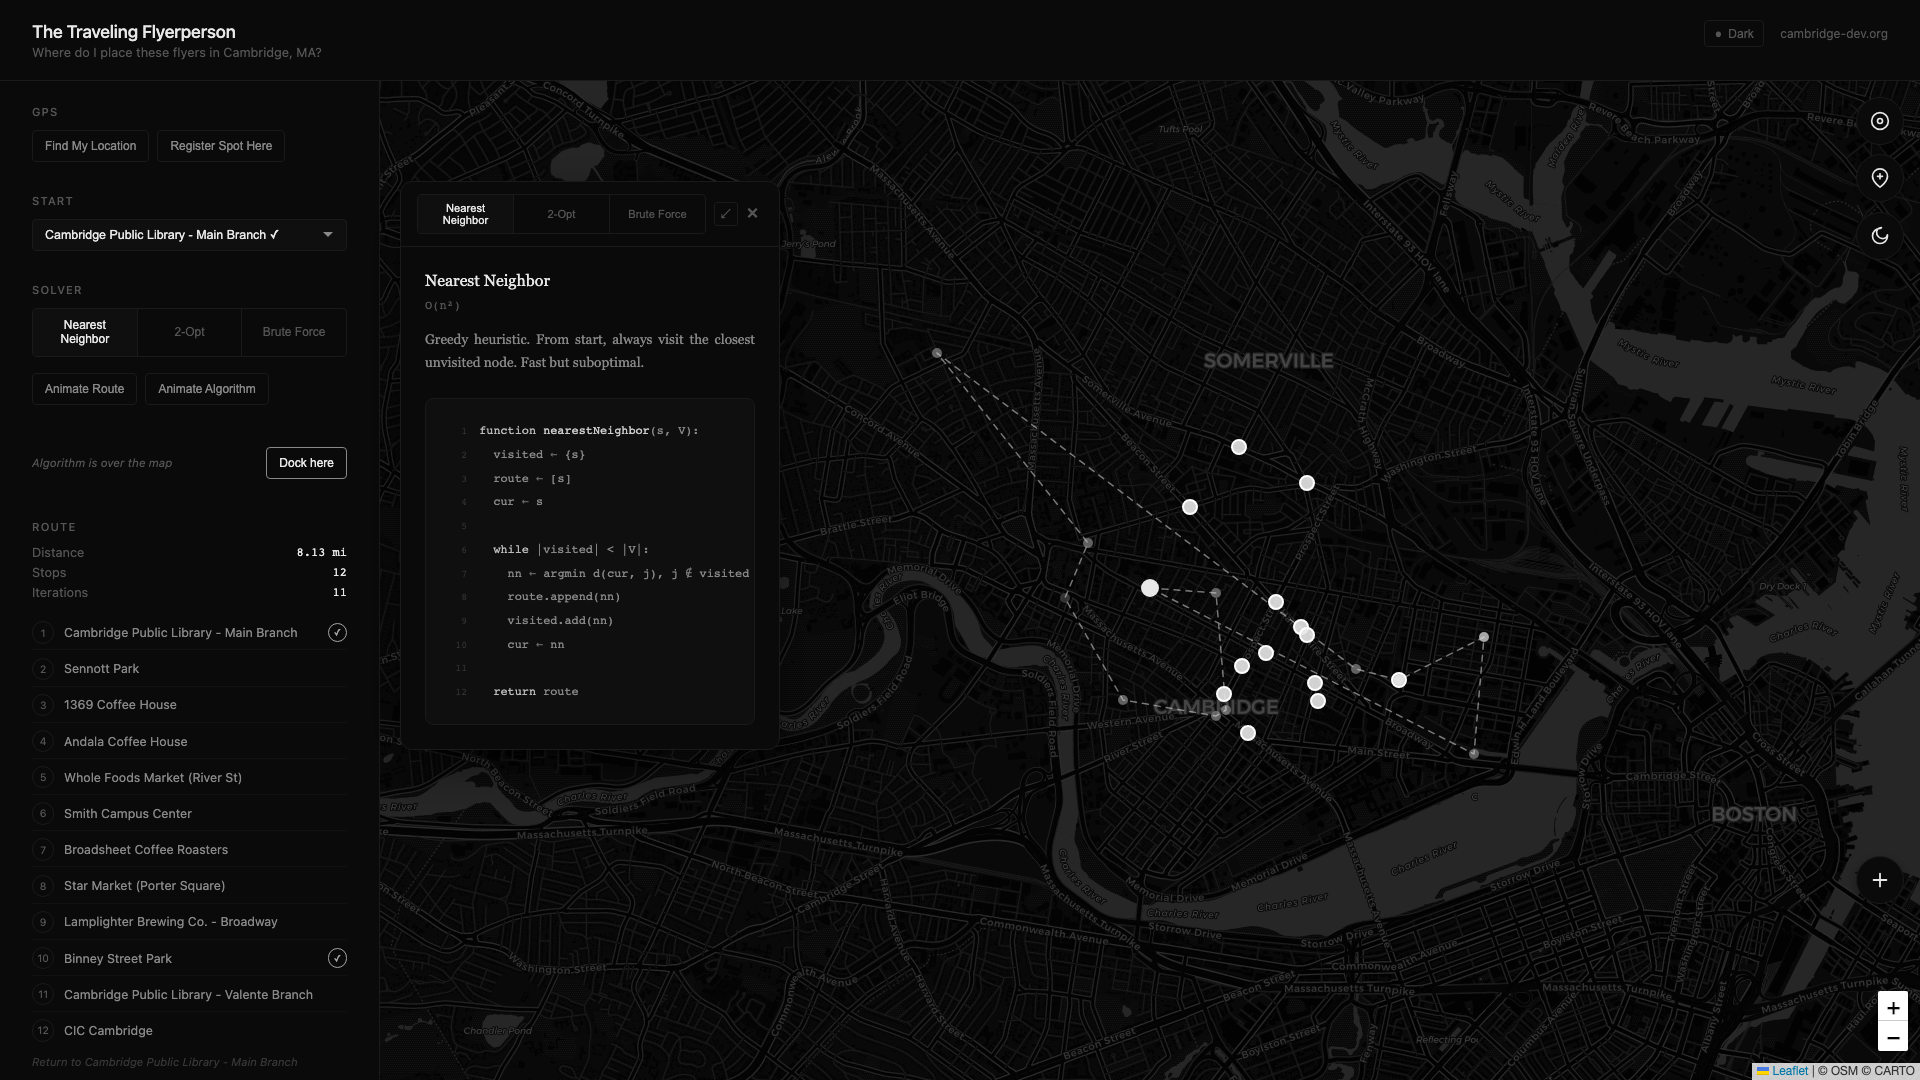
\includegraphics[width=\linewidth]{figures/app-desktop-2.png}
    \caption{The algorithm panel expanded over the map. Pseudocode is rendered with line numbers; the active line highlights as the route is built step by step, mirroring a debugger's stepping behavior.}
    \label{fig:algorithm}
\end{figure}

\begin{figure}[t]
    \centering
    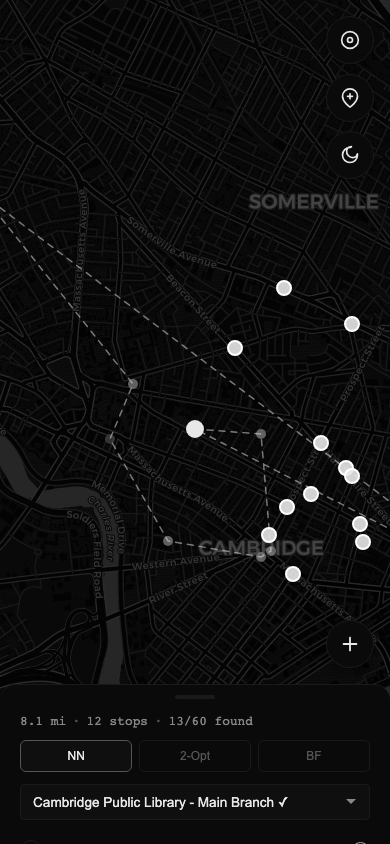
\includegraphics[width=0.55\linewidth]{figures/app-mobile.png}
    \caption{Mobile layout with bottom sheet and floating action buttons for field use.}
    \label{fig:mobile}
\end{figure}

Key features:
\begin{enumerate*}[label=(\arabic*)]
    \item Three solvers with animated, step-by-step execution showing pseudocode alongside the map
    \item Evidence registry: photographs of placed flyers, geotagged via EXIF metadata
    \item OpenStreetMap layers: traffic signals, bulletin board candidates (cafes, libraries, community centers), and transit stops
    \item Legal overlay: visual indication of which locations are legally constrained
    \item Mobile-first: swipeable bottom sheet, GPS integration, and floating action buttons for field use
\end{enumerate*}

The algorithm visualization is the application's primary pedagogical feature. Rather than treating the solver as a black box that returns a route, the app renders pseudocode with the active line highlighted as the algorithm executes---like stepping through a debugger. You can watch Nearest Neighbor greedily pick the next closest stop, or watch 2-Opt try and reject segment reversals in real time.

\section{What Makes This Interesting}

The routing problem is the entry point, but the deeper question is: \emph{which locations are actually worth visiting?} Route optimization assumes you already know where to go. The harder problem is figuring out where to go in the first place.

This leads to questions about:
\begin{description}
    \item[Survival] How long does a flyer last at a given location before it's removed or covered?
    \item[Exposure] How many people actually see and engage with a board at that location?
    \item[Learning] If you've never posted at a location before, how do you estimate its value from similar locations?
\end{description}

These questions are the subject of the companion paper, which develops a full Bayesian hierarchical framework combining survival analysis, spatial point processes, and multi-armed bandits. But the intuition is simple: a flyer on a busy transit shelter that gets removed in 6 hours is worth less than a flyer in a quiet laundromat that stays up for 3 months---even though the shelter has 100$\times$ more foot traffic.

\section{Current Status}

As of May 2026:
\begin{enumerate*}[label=(\arabic*)]
    \item 10 curated flyering locations across Cambridge
    \item 13 flyers placed and photographed
    \item An estimated 60 flyers in circulation city-wide
    \item Three working solvers with step-by-step animation
    \item A documented mathematical framework awaiting more observations
\end{enumerate*}

The project is intentionally small. It's a real task done by a real group, held to a standard of rigor that makes it useful as both a civic tool and a teaching artifact.

\section{What's Next}

\begin{enumerate*}[label=(\arabic*)]
    \item Real walking/biking distances via OSRM or GraphHopper
    \item Population density and foot traffic heatmap overlay
    \item Time-of-day simulation (morning commute vs. evening)
    \item Confirmed vs. estimated placement visualization
    \item Closing the loop: using collected evidence to update the predictive model
\end{enumerate*}

\section*{Links}

\begin{enumerate*}[label=(\arabic*)]
    \item Application: \url{https://letters-cambridge.web.app/stories/flyering/}
    \item Organization: \url{https://www.cambridge-dev.org/}
\end{enumerate*}

\end{document}
